% -*- fill-column: 80 -*-

\documentclass[11pt,a4paper,]{article}

\usepackage[margin=2.5cm]{geometry}
\usepackage[dvipsnames]{xcolor}
\usepackage{nicematrix,tikz}
\usepackage{parskip}
\usepackage{todonotes}
\usepackage{regexpatch}
\makeatletter
\xpatchcmd{\@todo}{\setkeys{todonotes}{#1}}{\setkeys{todonotes}{inline,#1}}{}{}
\makeatother
\usepackage{microtype}
\usepackage{extarrows}
\usepackage{amssymb,amsmath}
\usepackage{mathpazo}
\usepackage{longtable,booktabs}
\usepackage{dcolumn}
\usepackage{graphicx}
\usepackage{natbib}
\usepackage{hyperref}
\usepackage[capitalise,noabbrev,nameinlink]{cleveref}
\hypersetup{
  pdftitle={Ouroboros Leios simulation: building confidence in the performance results},
  pdfborder={0 0 0},
  breaklinks=true
}
\usepackage{subcaption}
\usepackage{listings}
\usepackage{minted}
%%\newcommand{\debug}[1]{}
\newcommand{\debug}[1]{#1}
\newcommand{\scenarioVsIdealFigure}[2]{
\begin{figure}[htbp]
    \centering
    \debug{\textbf{Label: #2} \\}
    \begin{subfigure}[b]{0.45\textwidth}
        \centering
        \includegraphics[width=\textwidth]{{#1}/IB-0.5-vs-ideal-vs-fitted-fig.eps}
        \caption{IB diffusion to $0.50$ stake.}
        \label{#1:ib0.5}
    \end{subfigure}
    \hfill
    \begin{subfigure}[b]{0.45\textwidth}
        \centering
        \includegraphics[width=\textwidth]{{#1}/IB-0.98-vs-ideal-vs-fitted-fig.eps}
        \caption{IB diffusion to $0.98$ stake.}
        \label{#1:ib0.98}
    \end{subfigure}
    
    \vspace{1em}
    
    \begin{subfigure}[b]{0.45\textwidth}
        \centering
        \includegraphics[width=\textwidth]{{#1}/EB-0.5-vs-ideal-vs-fitted-fig.eps}
        \caption{EB diffusion to $0.50$ stake.}
        \label{#1:eb0.5}
    \end{subfigure}
    \hfill
    \begin{subfigure}[b]{0.45\textwidth}
        \centering
        \includegraphics[width=\textwidth]{{#1}/EB-0.98-vs-ideal-vs-fitted-fig.eps}
        \caption{EB diffusion to $0.98$ stake.}
        \label{#1:eb0.98}
    \end{subfigure}
    
    \vspace{1em}
    
    \begin{subfigure}[b]{0.45\textwidth}
        \centering
        \includegraphics[width=\textwidth]{{#1}/VT-0.5-vs-ideal-vs-fitted-fig.eps}
        \caption{VT diffusion to $0.50$ stake.}
        \label{#1:vt0.5}
    \end{subfigure}
    \hfill
    \begin{subfigure}[b]{0.45\textwidth}
        \centering
        \includegraphics[width=\textwidth]{{#1}/VT-0.98-vs-ideal-vs-fitted-fig.eps}
        \caption{VT diffusion to $0.98$ stake.}
        \label{#1:vt0.98}
    \end{subfigure}
    
    \vspace{1em}
    
    \begin{subfigure}[b]{0.45\textwidth}
        \centering
        \includegraphics[width=\textwidth]{{#1}/RB-0.5-vs-ideal-vs-fitted-fig.eps}
        \caption{RB diffusion to $0.50$ stake.}
        \label{#1:rb0.5}
    \end{subfigure}
    \hfill
    \begin{subfigure}[b]{0.45\textwidth}
        \centering
        \includegraphics[width=\textwidth]{{#1}/RB-0.98-vs-ideal-vs-fitted-fig.eps}
        \caption{RB diffusion to $0.98$ stake.}
        \label{#1:rb0.98}
    \end{subfigure}

    \caption{Scenario \ref{#2}, diffusion latencies from slot start (300s run with default seed).}
    \label{fig:#1}
\end{figure}
}


\begin{document}

\title{Ouroboros Leios simulation: \\
building confidence in the performance results \\
{\large \sc An IOHK technical report}
}
\date{Version 1.0, April 2021}
\author{Andrea Vezzosi     \\ {\small \texttt{andrea@well-typed.com}} \\
\and Duncan Coutts      \\ {\small \texttt{duncan@well-typed.com}}
}

\maketitle

\section{Introduction}
\label{introduction}


\tableofcontents

\listoftodos

\section{Summary}
\label{summary}

\definecolor{Bu}{HTML}{069AF3}
\definecolor{Gn}{HTML}{15B01A}
\begin{center}
    \begin{NiceTabular}{c c c c c}[cell-space-limits=2pt,color-inside,rounded-corners]
        \CodeBefore
        \definecolorseries{BuGn}{rgb}{last}{Bu}{Gn}
        \resetcolorseries[\value{iRow}]{BuGn}
        \rowlistcolors{1}{BuGn!!+}
        \Body
        \Block[tikz = {left color=Bu, right color=Gn}]{*-*}{}
        \text{Most Idealised}
         &
        \multicolumn{3}{c}{\(\xleftrightarrow{\hspace{6cm}}\)}
         &
        \text{Most Realistic}
        \\
        \text{Scenario 1}
         &
        \text{Scenario 2}
         &
        \text{Scenario 3}
         &
        \text{Scenario 4}
         &
        \text{Scenario 5}
    \end{NiceTabular}
\end{center}

Most idealized setting for the simulation:
\begin{itemize}
    \item Nodes request block bodies from every peer.
    \item Mini-protocols are each run on a dedicated connection.
    \item The network model is a simplified one where packets are sent in-order and
          limited only by latency and bandwidth.
    \item An unbounded number of CPU intensive tasks, like validation, are simulated to run in parallel.
    \item Delays and sizes for blocks are kept uniform.
\end{itemize}

Scenarios proceed from most idealized and gradually turn one more realism feature:
\begin{enumerate}
    \item \label{sc:most-idealized} most idealized.
    \item \label{sc:request-from-first} nodes request block bodies from first peer available.
    \item \label{sc:multiplexing} mini-protocols are multiplexed over one connection.
    \item \label{sc:tcp} network layer more closely models TCP, in particular acks
          and congestion window collapse/restart.
    \item \label{sc:boundedcpu} nodes simulate CPU tasks with a finite number of worker threads.
    \item \label{sc:order} request IB bodies in oldest-first order.
\end{enumerate}
\todo{move Scenario \ref{sc:order} out of ordered list and into a ``variants'' list}
The last scenario is not strictly about realism, but we rather want to
investigate the impact of deviating from the freshest-first default.

\section{Scenario \ref{sc:most-idealized}}
\label{scenario1}
The least realistic scenario. Config:
\begin{minted}{yaml}
relay-strategy: "request-from-all"
tcp-congestion-control: false
multiplex-mini-protocols: false
treat-blocks-as-full: true
\end{minted}
In Figure~\ref{fig:scenario1} we compute ideal times two ways:
\begin{itemize}
    \item \textbf{ideal} -- Uses $3$ latencies for every communication.
    \item \textbf{ideal-fitted} -- Uses $3$ latencies for RB and EB, but $4$ for IB and $3.5$ for Votes.
\end{itemize}
we see that ideal-fitted better matches the simulation.

The Relay mini-protocol involves the consumer first requesting new headers, so
it can take $4$ latencies to receive the body. When blocks are more sporadic,
like for EBs and RBs, the consumer has likely already sent a blocking request
for more headers, so $3$ latencies are enough.
Votes all get sent at the start of the slice, with default configuration at least, so we can expect consumers to reach the blocking stage again by the next burst. However, due to the large traffic, the $4$ latencies path likely sees some use too. This mix of behaviours can explain the better fit using $3.5$ latencies.

\scenarioVsIdealFigure{scenario1}{sc:most-idealized}

\subsection{Uniform Voting stage}
The diffusion latencies, in Fig. \ref{fig:scenario1-send-recv}, stay very
similar when the simulation is set to generate votes across the whole stage
rather than only in the first slot.
From second $80$ to $300$ we have $\sim 1100$ vote messages, for an average of $\sim 5$
VT/s, same as IBs. The traffic pattern then does not seem a factor in the observed behaviour.
\begin{figure}[htbp]
    \centering
    \begin{subfigure}[b]{0.45\textwidth}
        \centering
        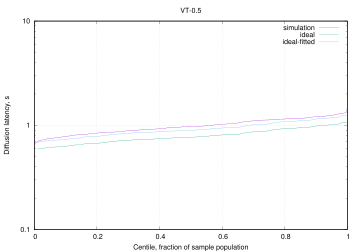
\includegraphics[width=\textwidth]{scenario1/VT-0.5-vs-ideal-vs-fitted-fig.eps}
        \caption{VT diffusion to $0.50$ stake.}
        \label{scenario1-send-recv:vt0.5}
    \end{subfigure}
    \hfill
    \begin{subfigure}[b]{0.45\textwidth}
        \centering
        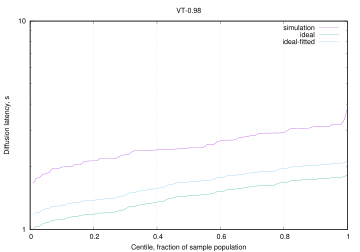
\includegraphics[width=\textwidth]{scenario1/VT-0.98-vs-ideal-vs-fitted-fig.eps}
        \caption{VT diffusion to $0.98$ stake.}
        \label{scenario1-send-recv:vt0.98}
    \end{subfigure}
    \caption{Scenario \ref{sc:most-idealized} with \textbf{uniform voting}, diffusion latencies from slot start (300s run with default seed).}
    \label{fig:scenario1-send-recv}
\end{figure}

\subsection{Large votes}
The diffusion latencies, in Fig. \ref{fig:scenario1-big-votes} and
\ref{fig:scenario1-big-votes-send-recv}, are collected for votes set to the size
of input blocks. With start-of-stage voting (the default) we see diffusion running
slightly slower than ideal with $4$ latencies, while uniform voting has a very
close fit. The delay in the former is possibly due to the $\sim 0.05s$
serialization time causing blocks to queue behind each other when they are all
generated at once: the volume of data, $102400*100$, is $5$ times the bandwidth
of any given link, and nodes are requesting bodies from everyone.

\begin{figure}[htbp]
    \centering
    \begin{subfigure}[b]{0.45\textwidth}
        \centering
        \includegraphics[width=\textwidth]{scenario1-big-votes/VT-0.5-vs-ideal-4-hops-fig.eps}
        \caption{VT diffusion to $0.50$ stake.}
        \label{scenario1-big-votes:vt0.5}
    \end{subfigure}
    \hfill
    \begin{subfigure}[b]{0.45\textwidth}
        \centering
        \includegraphics[width=\textwidth]{scenario1-big-votes/VT-0.98-vs-ideal-4-hops-fig.eps}
        \caption{VT diffusion to $0.98$ stake.}
        \label{scenario1-big-votes:vt0.98}
    \end{subfigure}
    \caption{Scenario \ref{sc:most-idealized} with \textbf{large votes, start-of-stage voting}, diffusion latencies from slot start (300s run with default seed).}
    \label{fig:scenario1-big-votes}
\end{figure}
\begin{figure}[htbp]
    \centering
    \begin{subfigure}[b]{0.45\textwidth}
        \centering
        \includegraphics[width=\textwidth]{scenario1-big-votes-send-recv/VT-0.5-vs-ideal-4-hops-fig.eps}
        \caption{VT diffusion to $0.50$ stake.}
        \label{scenario1-big-votes-send-recv:vt0.5}
    \end{subfigure}
    \hfill
    \begin{subfigure}[b]{0.45\textwidth}
        \centering
        \includegraphics[width=\textwidth]{scenario1-big-votes-send-recv/VT-0.98-vs-ideal-4-hops-fig.eps}
        \caption{VT diffusion to $0.98$ stake.}
        \label{scenario1-big-votes-send-recv:vt0.98}
    \end{subfigure}
    \caption{Scenario \ref{sc:most-idealized} with \textbf{large votes, uniform voting}, diffusion latencies from slot start (300s run with default seed).}
    \label{fig:scenario1-big-votes-send-recv}
\end{figure}

\section{Scenario \ref{sc:request-from-first}}
\label{scenario2}
Fig.~\ref{fig:scenario2}
\scenarioVsIdealFigure{scenario2}{sc:request-from-first}
\todo{compare to previous plot rather than ideal? Same for later sections.}

\section{Scenario \ref{sc:multiplexing}}
\label{scenario3}
Fig.~\ref{fig:scenario3} shows the result of multiplexing all the mini-protocols onto the same connection. We do not see a significant difference with Scenario~\ref{sc:request-from-first}.

Note that multiplexing in the simulation happens at the level of whole mini-protocol messages, without specific attempts to share the bandwidth fairly between them. This is not as realistic as breaking messages into same-size chunks and interleave those in a round-robin fashion.
\scenarioVsIdealFigure{scenario3}{sc:multiplexing}

\section{Scenario \ref{sc:tcp}}
\label{scenario4}
Fig.~\ref{fig:scenario4} shows the introduction of the tcp congestion window having a quite dramatic effect on diffusion times.
\scenarioVsIdealFigure{scenario4}{sc:tcp}
\todo{do IBs which do not reference RBs do better?}

As the bounded CPU scenario does better (see next section), we want to rule out the unbounded cpu task handler as problematic, but Fig.~\ref{fig:scenario4-100-cpu} is no better. So it seems actually limiting parallelism is what improves diffusion.
\scenarioVsIdealFigure{scenario4-100-cpu}{sc:tcp-100-cpu}

From other simulations we noticed there is a sweet spot of traffic for diffusion to do best, which makes sense with regard to keeping the congestion window open without overwhelming other resources. In particular from Fig.~\ref{fig:scenario4-best-IB-rate} we see IBs do slightly better with these parameters:
\begin{minted}{yaml}
ib-body-avg-size-bytes: 163840
leios-stage-length-slots: 60
ib-generation-probability: 10
\end{minted}
and a topology where link bandwidth is set to $1024000$ bps, half of previous scenarios.
\scenarioVsIdealFigure{scenario4-best-IB-rate}{sc:tcp-opt}

Fig.~\ref{fig:scenario4-higher-IB-rate} shows $15$ IBs per slot, rather than the $10$ of Fig.~\ref{fig:scenario4-best-IB-rate}, which flattens the curve even more, though we keep a substantial tail. On the other hand Vote diffusion is negatively affected, possibly crowded out by the IB volume.
\scenarioVsIdealFigure{scenario4-higher-IB-rate}{sc:tcp-higher-IB-rate}


In Fig.~\ref{fig:scenario4-higher-IB-rate-send-recv} we turn on uniform voting for the whole $60$s slot of the voting stage, which does appear to improve diffusion.
\scenarioVsIdealFigure{scenario4-higher-IB-rate-send-recv}{sc:tcp-higher-IB-rate-send-recv}

In Fig.~\ref{fig:scenario4-higher-IB-rate-send-recv-short-stage} we bring stage length back to the default $20$, and we see diffusion degrade again, though not to the original levels. About a tenth of IBs do not reach 0.98 stake distribution, and the curve flexes earlier than in Fig.~\ref{fig:scenario4-higher-IB-rate-send-recv}. Vote diffusion is also affected but not as much.
\scenarioVsIdealFigure{scenario4-higher-IB-rate-send-recv-short-stage}{sc:tcp-higher-IB-rate-send-recv-short-stage}


A possibility is that IBs are not fully diffusing because nodes are unable to reconstruct the ledger state to validate them in.
In Fig.~\ref{fig:scenario4-higher-IB-rate-send-recv-short-stage-no-cert} we try to see what happens when we require too many votes for EBs to certify, so the actual ledger state stays at Genesis. However IBs will still reference the most recent RB with a ledger state on the generating node, so other nodes will have to have adopted the same RB at some point.\todo{try setting the reference RB as always Genesis} Even with that caveat we see IB diffusion improve, getting quite close to the one with 60 slot stage length. Ledger state reconstruction does seem a significant factor, since when EBs are 3 times rarer (Fig.~\ref{fig:scenario4-higher-IB-rate-send-recv}), or here where they do not get certified, diffusion does better. Inspecting the logs we can further note that most IBs are validated immediately upon reception, meaning the ledger state was already available, and only a tiny fraction waits up to ~$3$s, meaning that the real impediment is that EBs can get certified even if a good percentage of nodes has not and will not validate some of the referenced IBs, because they lack the corresponding RB/ledger state.
\todo{Keep ledger-state only for the preferred chain.}
\scenarioVsIdealFigure{scenario4-higher-IB-rate-send-recv-short-stage-no-cert}{sc:tcp-higher-IB-rate-send-recv-short-stage-no-cert}

Fig.~\ref{fig:scenario4-higher-IB-rate-send-recv-short-stage-no-cert-100-cpu} confirms the above with the bounded cpu worker pool, with a much larger than needed bound.
\scenarioVsIdealFigure{scenario4-higher-IB-rate-send-recv-short-stage-no-cert-100-cpu}{sc:tcp-higher-IB-rate-send-recv-short-stage-no-cert-100-cpu}


In Fig.~\ref{fig:scenario4-lower-stage-length} we show that shorter stage length (20 slots) negatively affects even the case with 10 IBs per slot, even when we try to compensate with a shorter validation time.
\scenarioVsIdealFigure{scenario4-lower-stage-length}{sc:tcp-lower-stage-length}


In Fig.~\ref{fig:scenario4-20IB-small} we see that $15$ IB per second do not diffuse quite as well when they are only $96$kB, even with stage length of 60.
\scenarioVsIdealFigure{scenario4-20IB-small}{sc:tcp-15IB-small}


\section{Scenario \ref{sc:boundedcpu}}
\label{scenario5}
As mentioned before, we see in Fig.~\ref{fig:scenario5} that just using 5 cores per node, instead of unbounded, improves diffusion by a good amount, without need for higher traffic. Presumably the limits on CPU make it so traffic is more spread out and keeps the tcp window open.
\scenarioVsIdealFigure{scenario5}{sc:boundedcpu}
\todo{try the higher traffic variations above, the sweet spot presumably shifted}

In Fig.~\ref{fig:scenario5-10-cpus} we show results for $10$ cpu cores per node. Here we see all IBs making it to $0.98$ stake diffusion.
\scenarioVsIdealFigure{scenario5-10-cpus}{sc:boundedcpu-10-cpus}

\section{Scenario \ref{sc:order}}
\label{scenario6}
Fig.~\ref{fig:scenario6} shows the effect of oldest-first diffusion for IBs, which is null with these parameters. Trace debugging shows most of the time there is only one available body to request. \todo{try with higher traffic}
\scenarioVsIdealFigure{scenario6}{sc:order}

As we will be mostly looking at IB diffusion, Fig.~\ref{fig:oldest-vs-freshest} shows adoption for only IBs but for more stake fractions.
\begin{figure}[htbp]
    \centering
    \debug{\textbf{Label: oldest-vs-freshest} \\}
    \begin{subfigure}[b]{0.45\textwidth}
        \centering
        \includegraphics[width=\textwidth]{scenario6/IB-0.5-oldest-vs-freshest.eps}
        \caption{IB diffusion to $0.50$ stake.}
        \label{fig:oldest-vs-freshest:ib0.5}
    \end{subfigure}
    \hfill
    \begin{subfigure}[b]{0.45\textwidth}
        \centering
        \includegraphics[width=\textwidth]{scenario6/IB-0.6-oldest-vs-freshest.eps}
        \caption{IB diffusion to $0.60$ stake.}
        \label{fig:oldest-vs-freshest:ib0.6}
    \end{subfigure}

    \vspace{1em}

    \begin{subfigure}[b]{0.45\textwidth}
        \centering
        \includegraphics[width=\textwidth]{scenario6/IB-0.7-oldest-vs-freshest.eps}
        \caption{IB diffusion to $0.70$ stake.}
        \label{fig:oldest-vs-freshest:ib0.7}
    \end{subfigure}
    \hfill
    \begin{subfigure}[b]{0.45\textwidth}
        \centering
        \includegraphics[width=\textwidth]{scenario6/IB-0.8-oldest-vs-freshest.eps}
        \caption{IB diffusion to $0.80$ stake.}
        \label{fig:oldest-vs-freshest:ib0.8}
    \end{subfigure}

    \vspace{1em}

    \begin{subfigure}[b]{0.45\textwidth}
        \centering
        \includegraphics[width=\textwidth]{scenario6/IB-0.9-oldest-vs-freshest.eps}
        \caption{IB diffusion to $0.90$ stake.}
        \label{fig:oldest-vs-freshest:ib0.9}
    \end{subfigure}
    \hfill
    \begin{subfigure}[b]{0.45\textwidth}
        \centering
        \includegraphics[width=\textwidth]{scenario6/IB-0.98-oldest-vs-freshest.eps}
        \caption{IB diffusion to $0.98$ stake.}
        \label{fig:oldest-vs-freshest:ib0.98}
    \end{subfigure}

    \caption{Scenario \ref{sc:order}, diffusion latencies from slot start (300s run with default seed).}
    \label{fig:oldest-vs-freshest}
\end{figure}

Fig.~\ref{fig:oldest-vs-freshest-10-cpus} shows same comparison but with 10 cpus per node. Diffusion for the 0.98 stake fraction improves, but we still see no differences between the diffusion strategies.
\begin{figure}[htbp]
    \centering
    \debug{\textbf{Label: oldest-vs-freshest-10-cpus} \\}
    \begin{subfigure}[b]{0.45\textwidth}
        \centering
        \includegraphics[width=\textwidth]{scenario6-10-cpus/IB-0.5-oldest-vs-freshest.eps}
        \caption{IB diffusion to $0.50$ stake.}
        \label{fig:oldest-vs-freshest-10-cpus:ib0.5}
    \end{subfigure}
    \hfill
    \begin{subfigure}[b]{0.45\textwidth}
        \centering
        \includegraphics[width=\textwidth]{scenario6-10-cpus/IB-0.6-oldest-vs-freshest.eps}
        \caption{IB diffusion to $0.60$ stake.}
        \label{fig:oldest-vs-freshest-10-cpus:ib0.6}
    \end{subfigure}

    \vspace{1em}

    \begin{subfigure}[b]{0.45\textwidth}
        \centering
        \includegraphics[width=\textwidth]{scenario6-10-cpus/IB-0.7-oldest-vs-freshest.eps}
        \caption{IB diffusion to $0.70$ stake.}
        \label{fig:oldest-vs-freshest-10-cpus:ib0.7}
    \end{subfigure}
    \hfill
    \begin{subfigure}[b]{0.45\textwidth}
        \centering
        \includegraphics[width=\textwidth]{scenario6-10-cpus/IB-0.8-oldest-vs-freshest.eps}
        \caption{IB diffusion to $0.80$ stake.}
        \label{fig:oldest-vs-freshest-10-cpus:ib0.8}
    \end{subfigure}

    \vspace{1em}

    \begin{subfigure}[b]{0.45\textwidth}
        \centering
        \includegraphics[width=\textwidth]{scenario6-10-cpus/IB-0.9-oldest-vs-freshest.eps}
        \caption{IB diffusion to $0.90$ stake.}
        \label{fig:oldest-vs-freshest-10-cpus:ib0.9}
    \end{subfigure}
    \hfill
    \begin{subfigure}[b]{0.45\textwidth}
        \centering
        \includegraphics[width=\textwidth]{scenario6-10-cpus/IB-0.98-oldest-vs-freshest.eps}
        \caption{IB diffusion to $0.98$ stake.}
        \label{fig:oldest-vs-freshest-10-cpus:ib0.98}
    \end{subfigure}

    \caption{Scenario \ref{sc:order}, diffusion latencies from slot start (300s run with default seed).}
    \label{fig:oldest-vs-freshest-10-cpus}
\end{figure}

\addcontentsline{toc}{section}{References}
\bibliographystyle{plainnat}
\bibliography{sim-realism}

\end{document}
